\section{提案するサーバテスト手法}

構成管理ツール独立性とOS・ディストリビューション汎用性をいかに満たすかを考察する.

特定の構成管理ツールからの独立性を満たせない理由は2つある.ひとつは構成管理ツールがもつOS・ディストリビューション汎用性を利用するために,テストの実装が特定の構成管理ツールに依存していることである.

もうひとつはテストスイートでのテスト用VM構築フェーズが,特定の構成管理ツールのみ対応していることである.

OS・ディストリビューション汎用性が満たせないのは,テストがシェルコマンドを直接記述する実装になっており,OS・ディストリビューションの違いをテストコードを書く者自らが意識しないといけないからである.

この考察から,提案するテスト手法に必要な要件は以下の通りとなる.

\begin{enumerate}
  \item テストの実装を特定の構成管理ツールに依存しない
  \item テストスイートではなくテストのみに特化する
  \item OS・ディストリビューションの違いを利用者に意識させない
\end{enumerate}

そこでまずOS・ディストリビューション毎にコマンドを分離し,統一的なAPIでコマンドを呼び出すことができる汎用コマンド実行フレームワークを定義する.このフレームワークではまず構成管理ツール固有の振る舞い(パッケージインストール等)を抽出する.そして振る舞いをテストするためのAPIを定義する.更にAPIから呼び出されるコマンドをOS・ディストリビューション毎に定義する.APIとコマンド群の間にはOS・ディストリビューションを判別して自動で適したコマンドを返すレイヤーを設ける.

次に,テストコードの記述の抽象性を高め可読性を上げるために,宣言的な記法で汎用コマンド実行フレームワークを操作できる制御テストフレームワークを定義する.このフレームワークではまず記法の定義を行う.次に記法内の各命令と実際に呼び出す汎用コマンド実行フレームワークのAPIメソッドをひもづける.

汎用コマンド実行フレームワークと制御テストフレームワークの仕組みおよびその関係を\figref{fig:framework}に示す.

\begin{figure}[tb]
  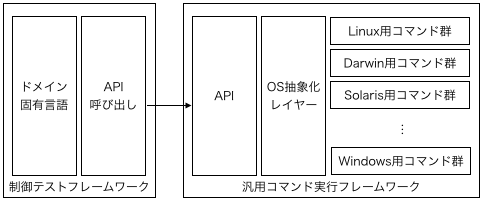
\includegraphics{framework-overview.png}
  \caption{汎用コマンド実行フレームワークと制御テストフレームワークの仕組みと関係}
  \label{fig:framework}
\end{figure}

この手法に基づき実装した汎用コマンド実行フレームワークをSpecInfra\cite{specinfra},制御テストフレームワークをserverspec\cite{serverspec}と名付けた.

SpecInfraとserverspecの実装の一部を示す.SpecInfraでは各OS用のコマンド群をクラスとして定義する.例としてRedHat系Linux上で指定されたパッケージがインストールされているかどうかを確認するコマンドの定義を\figref{fig:check-installed-on-redhat}に示す.また,Solaris上で指定されたパッケージがインストールされているかどうかを確認するコマンドの定義を\figref{fig:check-installed-on-solaris}に示す.serverspec上でこのコマンドを呼び出して指定したパッケージがインストールされているかどうかテストする部分の実装を\figref{fig:call-check-install}に示す.

\begin{figure}[tb]
\setbox0\vbox{
\begin{verbatim}
module SpecInfra::Command
  class RedHat < Linux
    def check_installed(package,version=nil)
      cmd = "rpm -q #{escape(package)}"
      if version
        cmd = "#{cmd} | grep -w -- #{escape(version)}"
      end
      cmd
    end
  end
end
\end{verbatim}
}
\centerline{\fbox{\box0}}
\caption{パッケージがインストールされているかを確認するRedHat系Linux用コマンド定義\label{fig:check-installed-on-redhat}}
\end{figure}

\begin{figure}[tb]
\setbox0\vbox{
\begin{verbatim}
module SpecInfra::Command
  class Solaris < Base
    def check_installed(package, version=nil)
      cmd = "pkg list -H #{escape(package)}"
      if version
        cmd = "#{cmd} | grep -qw -- #{escape(version)}"
      end
      cmd
    end
  end
end
\end{verbatim}
}
\centerline{\fbox{\box0}}
\caption{パッケージがインストールされているかを確認するSolaris用コマンド定義\label{fig:check-installed-on-solaris}}
\end{figure}


\begin{figure}[tb]
\setbox0\vbox{
\begin{verbatim}
module Serverspec::Type
  class Package < Base
    def installed?(provider, version)
      backend.check_installed(@name, version)
    end
  end
end
\end{verbatim}
}
\centerline{\fbox{\box0}}
\caption{パッケージインストールチェックコマンドを呼び出す部分のservespecでの実装\label{fig:call-check-install}}
\end{figure}

これらの実装の上で,サーバ上にntpパッケージがインストールされているかどうかを確認するためのテストコードをserverspecの記法で記述したものを\figref{fig:test-code-to-check-ntp-package-installed}に示す.

\begin{figure}[tb]
\setbox0\vbox{
\begin{verbatim}
describe package("ntp") do
  it { should be_installed }
end
\end{verbatim}
}
\centerline{\fbox{\box0}}
\caption{ntpパッケージがインストールされているかをテストするserverspecで記述したテストコード\label{fig:test-code-to-check-ntp-package-installed}}
\end{figure}
